\section{Trend analysis}

\subsection{Data Preprocessing}
\subsubsection{Data Format}
As described in the READ.ME of data provided, The targeted data is from the Korean Herald, National Section news. The period of the dataset is from 2015 to 2017. The Crawled date of the dataset is 2018-10-26. Data format is Json, and there are total of 6 data headers - title, author, time, description, body, and section. Total of 23769 news are included in this dataset.

\subsubsection{Load Data}
In order to load the data, the instructions recommended at READ.ME are followed. Pandas library is used for better storing and access of the news text.
\subsubsection{Libraries Used}
For this project, we used pandas, gensim, nltk, and neuroner python libraries. The install requirements are found on install.sh of the github repository.


\subsection{Previous approaches}
Issue trend analysis can be seen as a part of Topic modeling. By searching fields of recent Topic modeling, LDA has shown to have good performance. As a result, LDA is used as a baseline algorithm for this project.
A recent study(2018) on Topic Modeling shows that Topic Quality improves when Named Entities are promoted.\cite{krasnashchok-jouili-2018-improving} This paper proposes 2 techniques: 1. Independent Named Entity Promoting and 2. Document Dependent Named Entity Promoting. Independent Named Entity Promoting promotes the importance of the named entities by applying scalar multiplication alpha to the importance of the named entity word. Document Dependent Named Entity Promoting promotes the importance of the named entities by setting the weights of the named entities as maximum term-frequency per document. For Independent Named Entity Promoting, the value of alpha can be changed flexibly, but results conducted by this paper shows that setting alpha as 10 showed the best results.
We take advantage of this paper's idea on Independent Named Entity Promoting and implement Named Entity Promoted Topic Modeling by LDA.
\subsection{Experiments}
\subsubsection{Data Tokenization}
Several attempts were taken before we finalize the way Tokenization was done. Doing lemmatization was not always good.
At first try, Lemmatization(converting words into base forms) and removal of stopwords were conducted before we run the LDA algorithm and extract Named Entities. We thought that converting words into base forms and reducing the total vocabulary size would increase the performance of topic modeling. Stopwords were taken from nltk.corpus.stopwords.words("english"), and lemmatization functon was taken from
gensim.utils.lemmatize.
\mintinline{python}{res.append(lemmatize(raw\_text, stopwords=stopwords))}. But after we do lemmatization, remove stopwords, and tokenize the data, no Named Entities were extracted from the preprocessed corpus. We think the reason for this is as follows. 
First, words are all converted into lower case when we do lemmatization. This makes the Named Entitiy Recognition system(NER system) to work poorly because we have removed some of the original information(i.e. Upper case information), and word that starts with an upper case has a high probability that it is a "Proper pronoun", or "Unique word". We lose this sign of information.
Second, words are transformed into their base forms, limiting NER system to detect specific words. There also could be cases that the words are transformed into meanings other then their original meanings. For example, "Cooking" and "Cooker" are both converted into "cook" when they are lemmatized, and this makes the word to lose the original information.
Third, original relationships between words are lost, because of the removal of stopwords. When we do NER, we have to do the POS tagging of the sentence and then input both the word sequence and the POS sequence of the text. But when we artificially remove stopwords and then do NER, original relationships between words are disrupted and broken. This limits NER system to perform well.

For these 3 reasons, we decided to not apply lemmatization for tokenization, because lemmatization lose information about the original text. We decided to just use word\_tokenize from nltk.tokenize, do POS tagging and then do NER.


\subsubsection{Extract NER}
By using ne\_chunk from nltk and pos\_tag from nltk.tag, we extracted Named entities from the original news dataset. NER also extracts multi-word information of Named Entities other than just classifying whether a word is a named entity or not, so we decided to use that information. We store single-word Named Entities and multi-word Named Entities separately. As a result, NER and multi-word extraction of NER are both processed.

Below figure is the topic modeling result(of all time lengths from 2015 to 2017) WITH NER Promoting and WITHOUT NER Promoting. We can see the difference between those two results, and we can conclude topic modeling with NER promoting shows better performance.
\begin{figure*}[t]
    \centering
    \begin{subfigure}[b]{0.4\textwidth}
        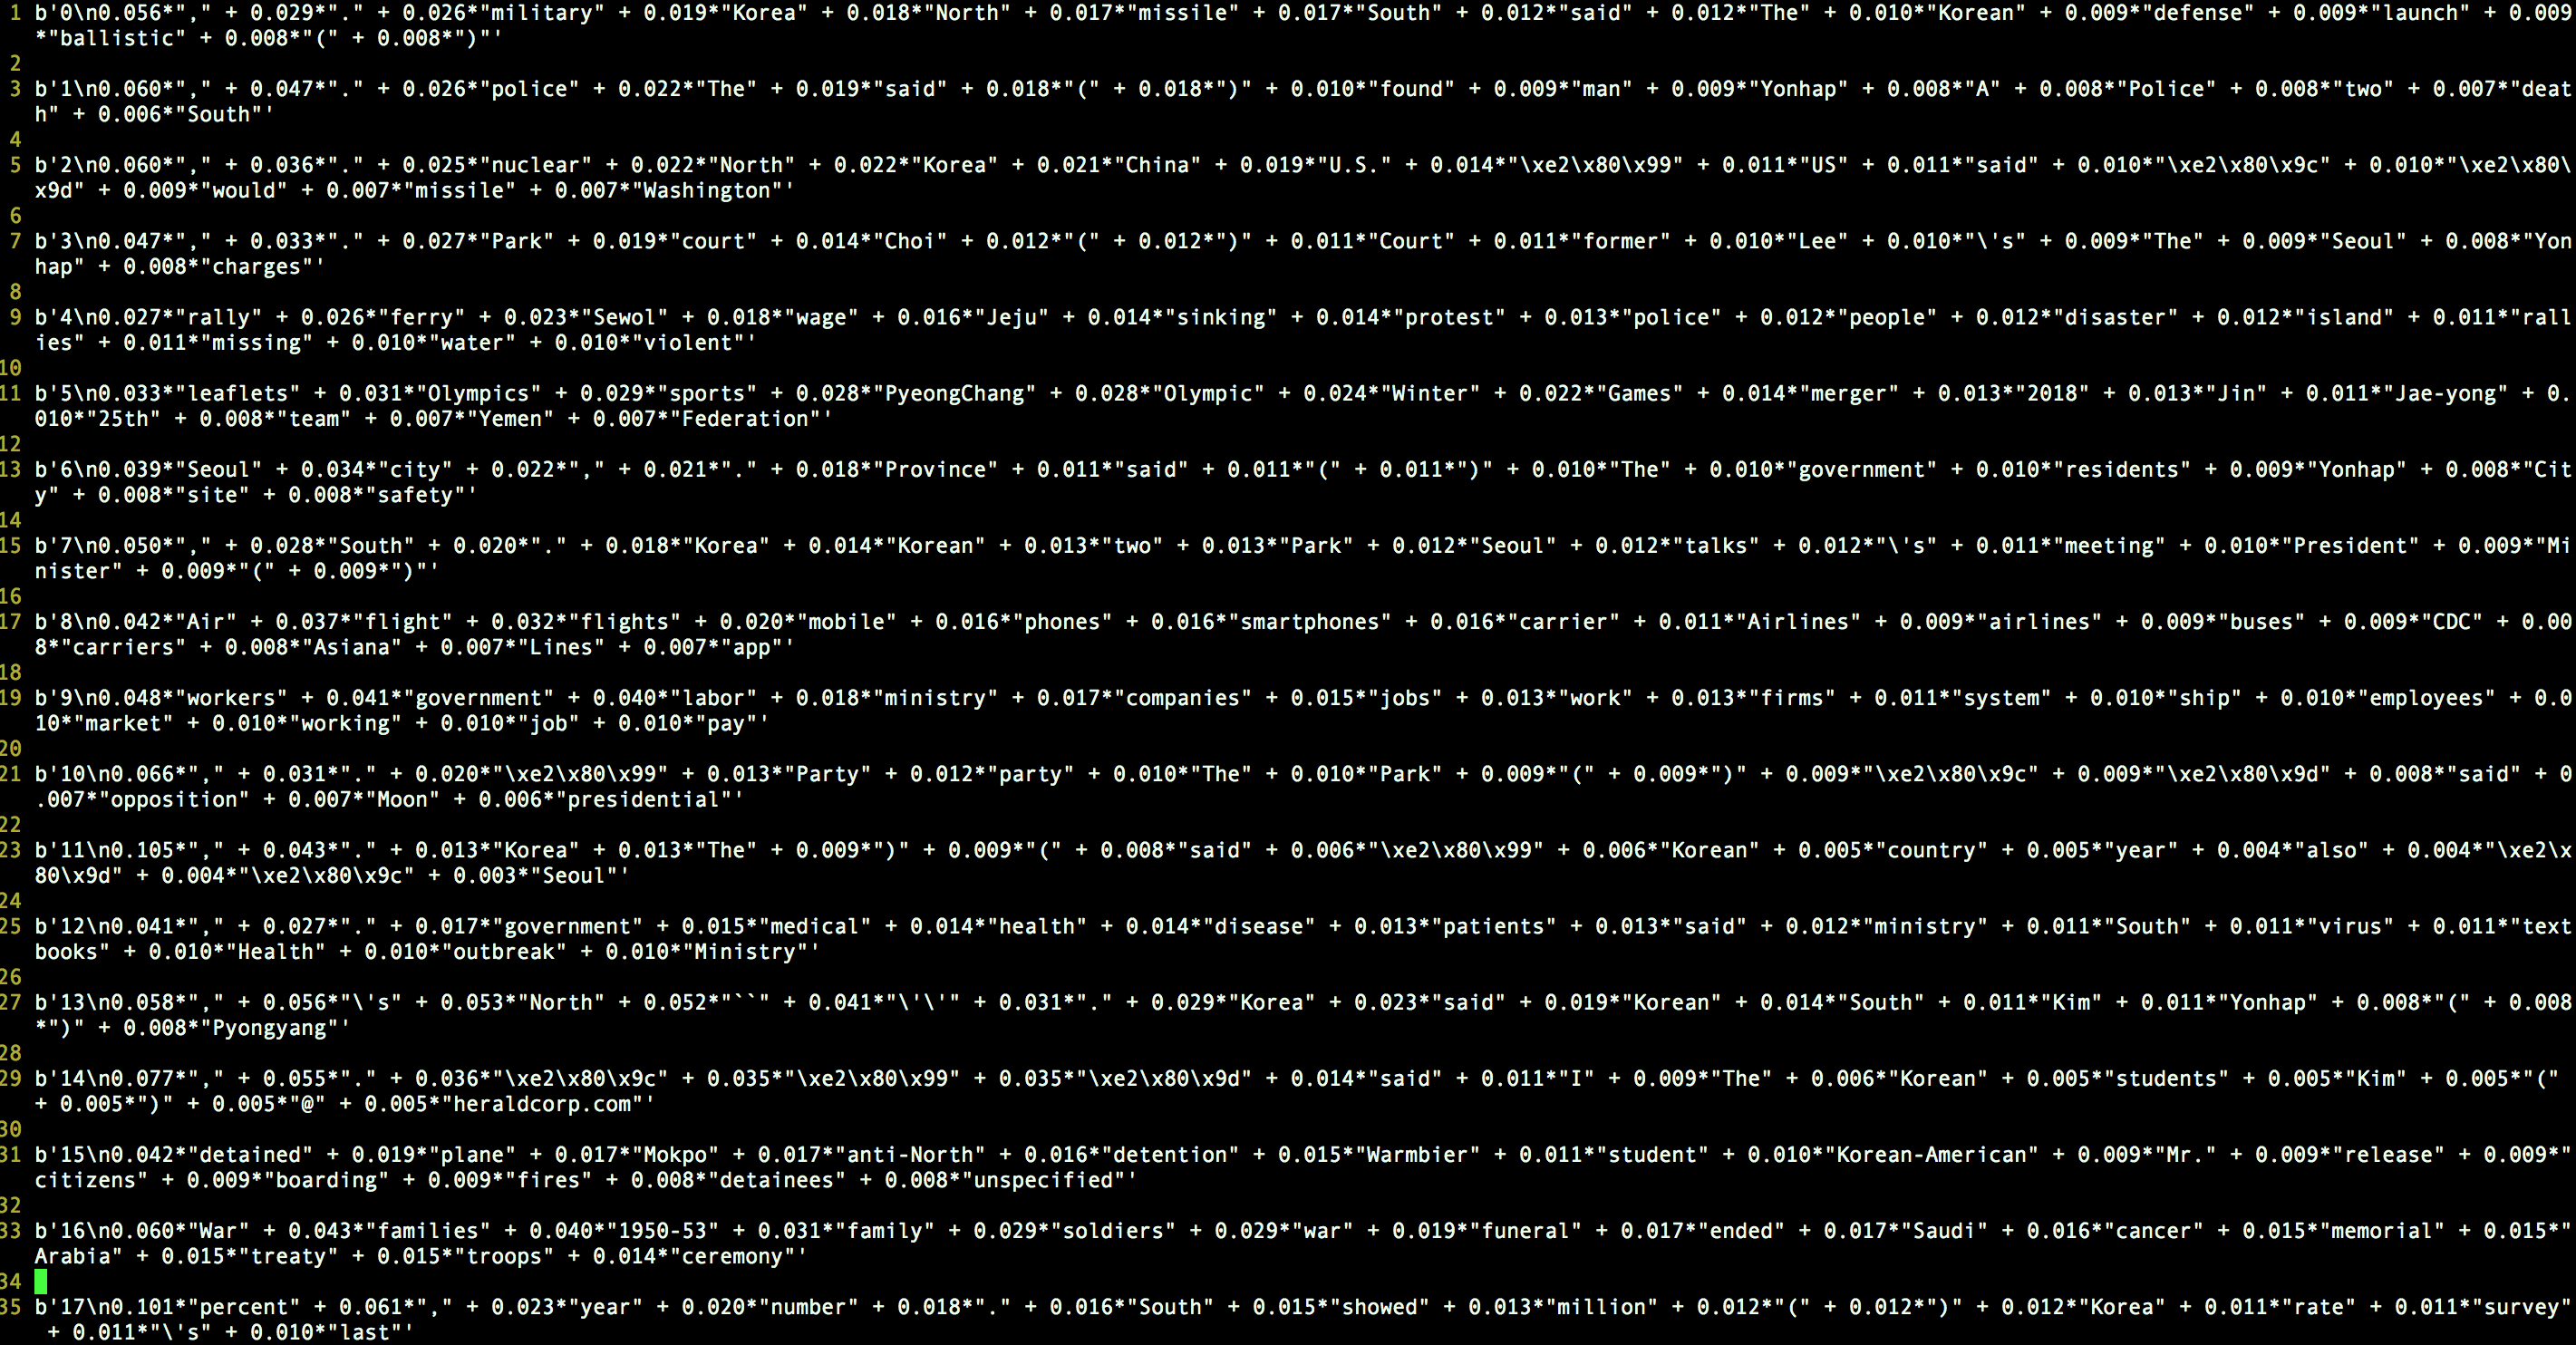
\includegraphics[width=\linewidth]{before_ner.png}
    \end{subfigure}
    \begin{subfigure}[b]{0.4\textwidth}
        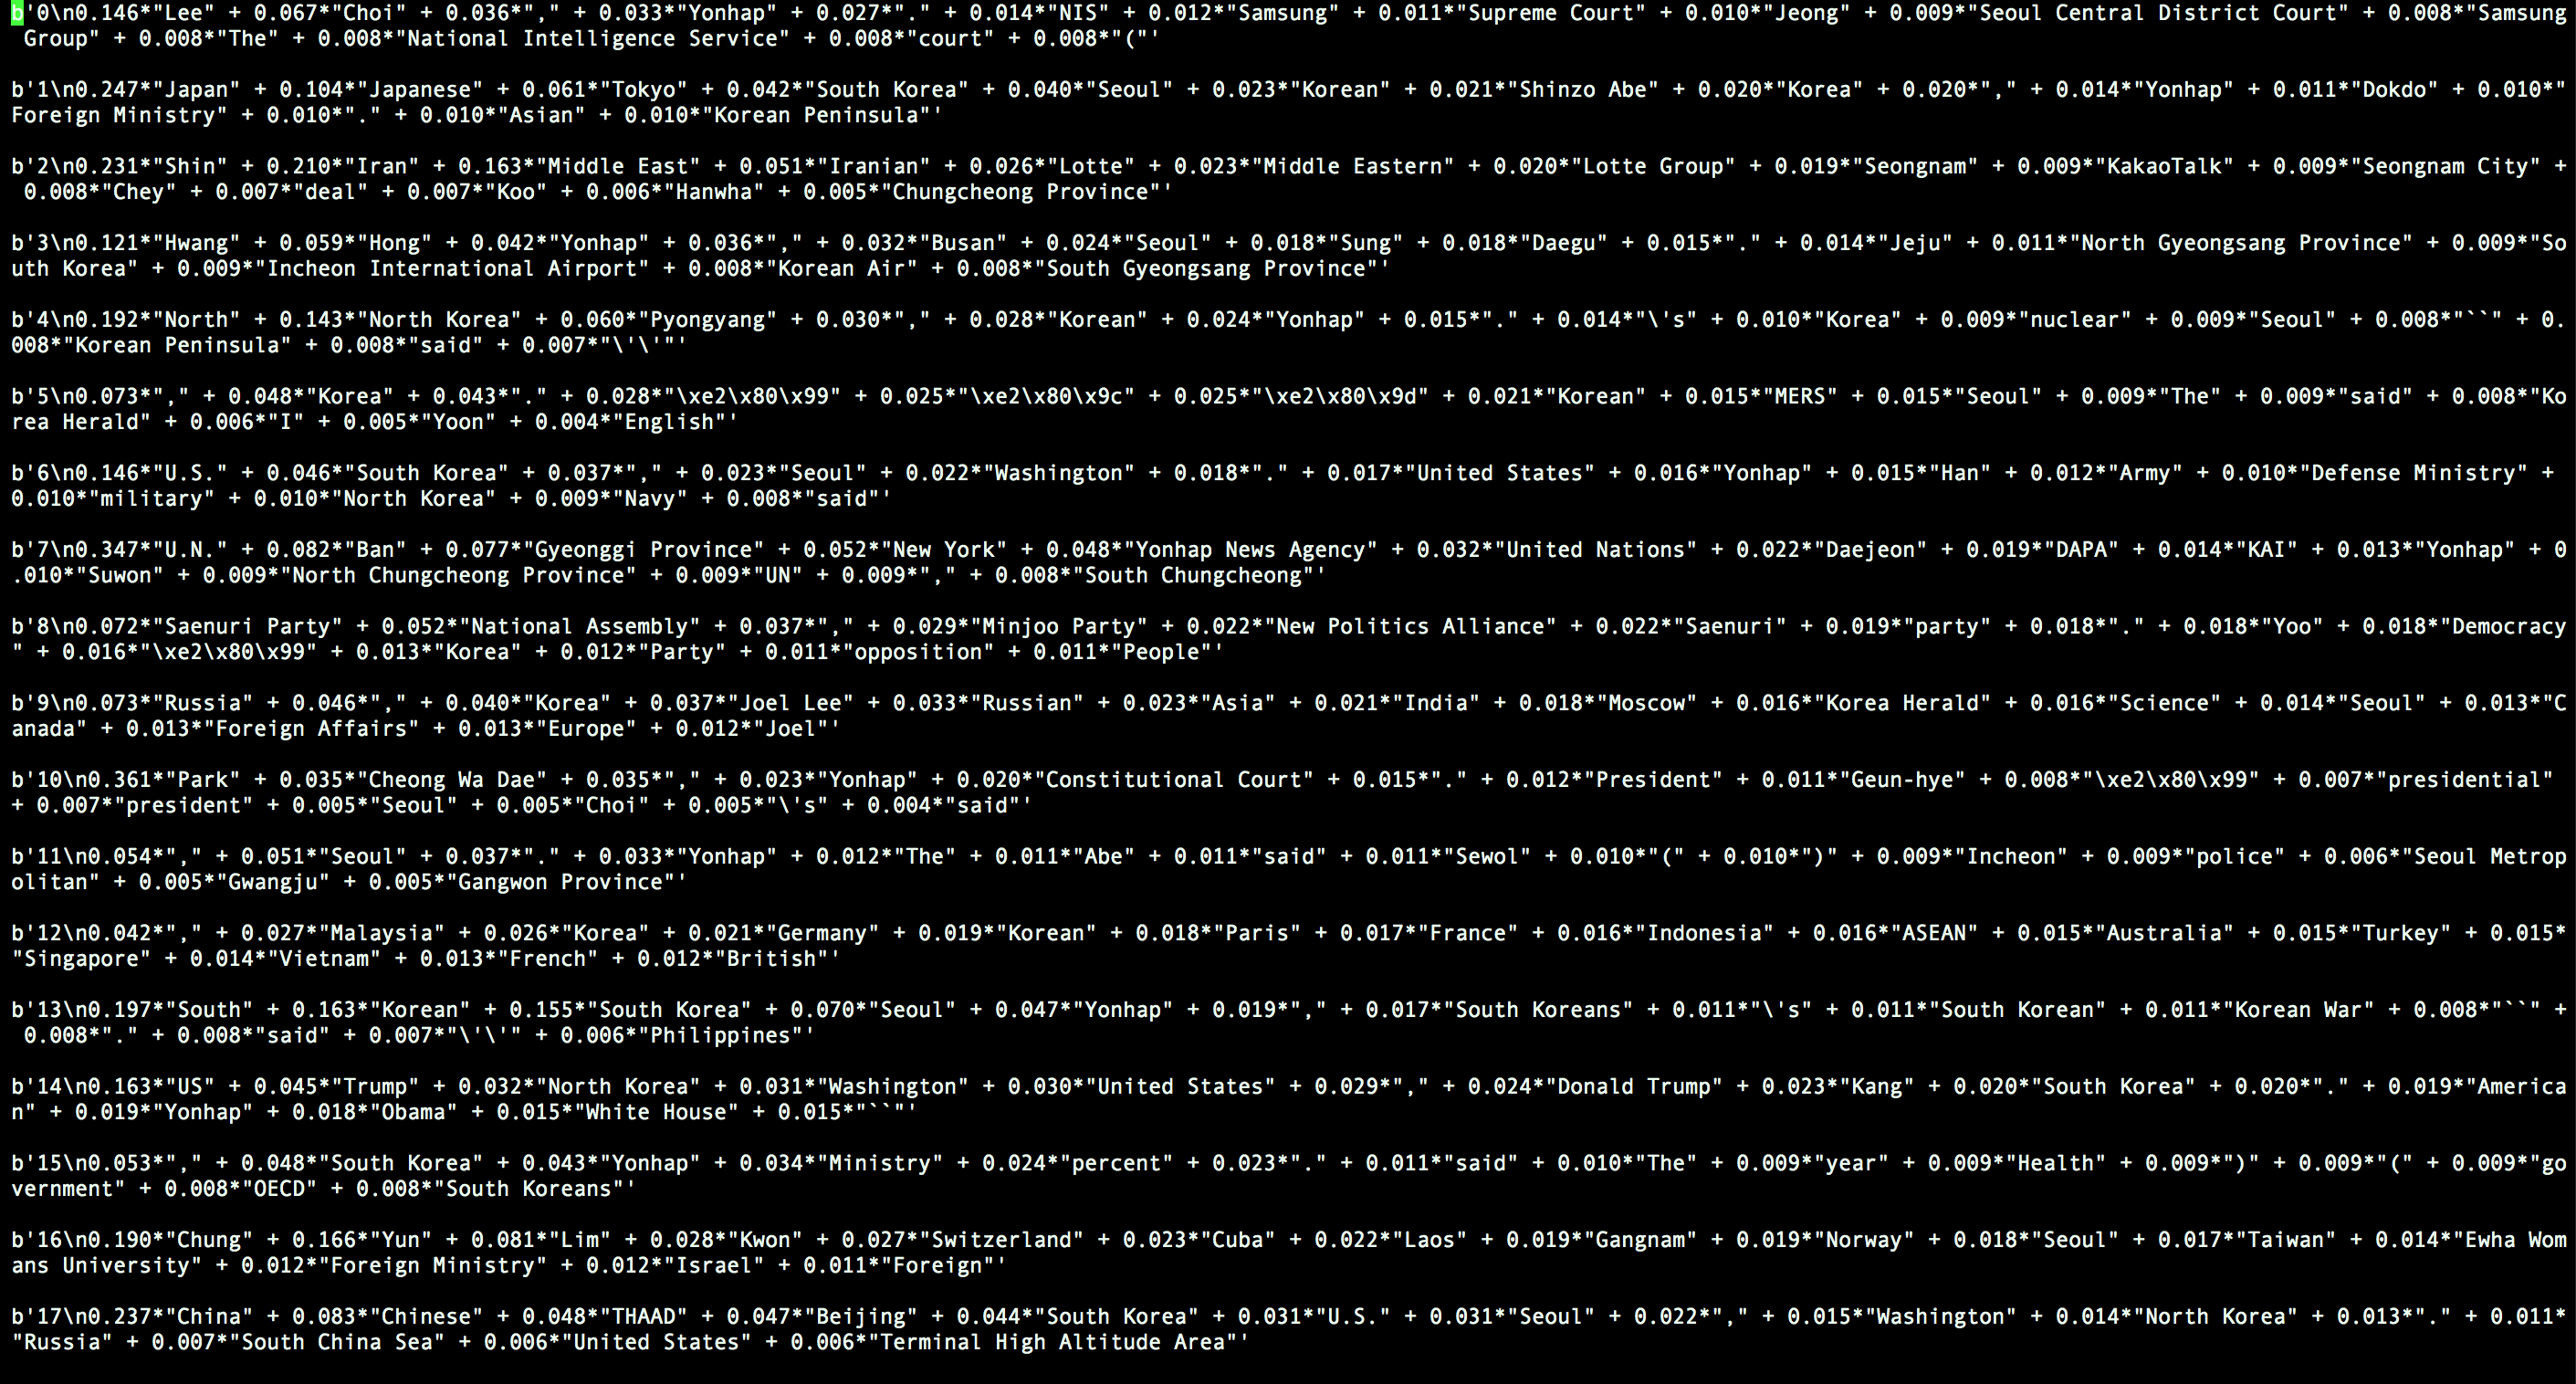
\includegraphics[width=\linewidth]{after_ner.png}
    \end{subfigure}
	\caption{Topic modeling result before/after NER}
\end{figure*}

\subsubsection{Improvement - apply neuroNER instead of nltk's Named Entity Recognition.} 
The topic modeling paper that we referenced used neuroNER for Named Entity Recognition. NeuronNER is an easy-to-use program for named entity recognition based on neural networks presented in emnlp 2017. \cite{2017neuroner} This neuroNER tool is trained on CONLL2003 dataset and recognizes four types of NE: person, location, organization and miscellaneous. NeuroNER also extracts multi-word information, so we use this multi-word information just as the previous NER did. Instead of using
\mintinline{python}{ne_chunk(pos_tag(preprocessed_text), binary=True)}, we change NER extraction to use below.

\begin{minted}{python}
nn = neuromodel.NeuroNER(train_model=False, use_pretrained_model=True)
nn.predict(preprocessed_text)
\end{minted}
to extract Named Entities from the text.

\subsubsection{Run LDA with neuroNER promoting.}
First, we split the dataset each year. Then, get tokens for each document with promoted NER frequency (X 10). With this corpus, run the LdaModel with num\_topics of 10 and num\_words of 30 to 50. At first try, we directly ran LDA on NER boosted news dataset. but with this approach, we found out that stopwords are classified as top(important)words according to the result of LDA. So we decided to remove stopwords after all the preprocssing(including NER weight promoting)are done. The timing of removal of stopwords are important, as removing stopwords before NER will affect the NER result(Removal of stopwords before POS Tagging will affect the POS Tagging result). Stopword removing are done right before feeding the tokens into LDA. After the removal of stopwords, we could see that the results were much better.

\subsubsection{Tuning LDA hyperparameters}
We set num\_topics to 10 for LDA becuase we need to extract top 10 important issues from each year. At first, we decided to train the LDA model with num\_topics of 10 and num\_words of 15. But the results were not very explainable. Also, the only removed word was the stopword after tokenization. Therefore non-ascii character, or unrelated words such as
\mintinline{python}{" \xec ' ( ) . ,} were introduced in the topic result. To extract useful information, we removed those unuseful information and increased num\_words for each topics to 50 to see more related words including each topic. First we set chunk\_size to 2000, num\_iterations to 4000, and alpha to 'auto'. We changed chunk\_size to 4000 and increased num\_iterations, and see if the result improved. But there was no significant change on the results. We finally decided to set num\_topics to 10, chunk\_size to 4000, iterations to 500, and passes to 30.

\subsubsection{TroubleShooting}
In order to increase the performance of Topic modeling, various approaches were taken. The first trial was to divide news dataset into given sections then do LDA modeling for each year, for each topic. But this approach can not detect the top 10 trending issues. Increasing the total topic size to more than 10 makes us difficult to analyze which topic is the top 10 most trending topic. This happened to be the same problem when we increase the total topic\_size to more than 10.
But, setting the total topic\_size to 10 also has problems. By setting the total topic\_size to 10 for each year, many topics can be concatenated into one. For this case, we filter out the majority topic by looking at the extracted tokens for each topic. Also, for the herald dataset, words related for "Korea" (Korean, North Korea, South Korea, Korean, ... ) are used very frequently accross all topics, so the Topic analysis result for this also showed great frequency of words related to "Korea", making "Korea" unuseful for topic detection. Also there were topic clusters that were hard to analyze the keyword. Also, NER was good at extracting \textbf{multi-words}, but was not good at extracting \textbf{triple or more words}. For example, the neuroNER output of "Moon Jae-in eat food" was "Moon Jae", not 'Moon Jae-in". We could see the inherent limitations when we try to extract 2 or more words just by using NER. To overcome those problems, more data preprocessingand multi-word extraction should be done. Also, If we link the corresponding news article that best represent a particular topic, it will make Topic modeling result more analyzable.

